\chapter{Communication protocol, state synchronization and future work}
\label{chap:proto}
This chapter is dedicated to the specification, design and implementation criteria of what will be referred to as the Distributed Group Creation Protocol (DGCP).
While in the previous chapters it has been suggested an algorithm for how groups can be formed, in this chapter the focus shall be on the technology and protocols required
to enable communication between access points, - and ultimately groups. There has already been done some work on the subject of access point communication over IP,
and previous work in the field of distributed consensus can be used to ensure synchronized group states. In this chapter these technologies will be covered and considered,
and finally a protocol sketch that stitches all required components together will be suggested. 


\section{Problem overview}
In chapter \ref{chap:clustering} we looked at an algorithm that enables cluster formation in a distributed environment where no node knows the complete layout of the surrounding networks.
A number of assumptions were made before we suggested an algorithm. Two of the assumptions encapsulated the three following problems:
\begin{itemize}
\item Direct contact between access points is possible
\item An underlying group communication protocol is in place
\item The state of a group is synchronized throughout all its members
\end{itemize}
In this chapter we shall attempt to handle these issues to create a more complete scheme for group creation in a distributed environment.

\section{Enabling technologies}
When designing a protocol that enables group communication, there is need for some some already well-researched theory and technology as a foundation. There are already enough
considerations to take when designing an architecture like this, and there is no need to reinvent the wheel where there is already done a good amount of research. 
Raft will be used for state synchronzation. Raft is a distributed consensus protocol and provides the equivalent degree of fault-tolerance as the Paxos \cite{lamport2001paxos} protocol family.
ResFi is a protocol used to enable communication over IP between adjacent access points. This section is dedicated to briefly introduce these protocols. 

\subsection{Distributed consensus with Raft}
Raft \cite{raftio} is a distributed consensus protocol designed with simplicity in mind. The creators of Raft designed it to be used for educational purposes. Traditionally, Paxos has been used to explain
distributed consensus, but Paxos has a complex design with extremely many different variations. Raft is now taught in courses all over the U.S, and their GitHub page includes to links
of implementations in a large amount of languages.

\subsection{Why distributed consensus?}
Distributed consesus can be beneficial for the distributed group creation protocol for a couple of reasons, the most important two being:
\begin{itemize}
	\item Leader election for decision making
	\item	Synchronous data replication (makes sure all nodes have a consistent picture of the group, in-case leader goes down)
\end{itemize}

\subsection{What Raft can not help with}
Raft is not originally intended to run in a flexible environment where the amount of servers changes rapidly. Hence Raft would not handle regrouping after a merge within the same Raft session.
There can be no consensus on "past" logs, as all groups will have different logs from before the merge. There is also no native method to invoke native leader handover, so in the event
of merge there would be two leaders. 

Another aspect that would be different from regular distributed consensus is the regular assumption that there are two main actors with different roles. Servers and clients. Servers are
supposed to hold synchronized data, replicated across all the servers. The clients are the actors who invokes changes on the data.

A traditional scenario is the banking example, where a client could be a mini-bank issuing a withdrawal from a bank account. The servers would be all the banking servers making sure the new,
updated account balance is consistent no matter where money is withdrawn from. 

In the distributed group creation protocol all nodes running Raft are both servers and clients. They have to report new changes in the form of neighbours and signal strength values,
while also keeping a local, replicated copy of the state of the group.

\subsection{Access point communication with ResFi}
This subsection is dedicated to briefly describe how ResFi operates, and to cover why and how it is a protocol that can be taken advantage of in the Distributed Group Creation Protocol. 

ResFi is a protocol framework that supports creation of radio resource management in legacy residential networks. ResFi is intented to be used in  a chaotically deployed landscape of acccess points,
which is similar to the intentions of the group creation in this thesis. It enables the creation of secure point-to-point communication channel over IP through wired backhaul network. 
Point-to-point in this context means APs that are directly adjacant (or neighbouring APs as it has been referred to in the group creation chapter).
It also supports secure broadcast via n-hop communication. A brief account of the sequential steps of the ResFi standard mode of operation follows,
the more thorough explanation can be find in the ResFi paper \cite{resfi} under chapter \textit{IV. Detailed Specification}.

\begin{enumerate}
	\item When an AP ($a$) is booted, a symmetric group key is created, along with an RSA key-pair. 
	\item $a$ scans all 802.11 channels for neighbouring APs. For each AP it finds, $a$ sends out a probe request that contains its public IP and public RSA key. It also includes
		the symmetric group key. As a response to the probe request it receives a probe response containing the equivalent information for each neighbour. 
	\item When the exhchange has happened, $a$ subscribes to the publish sockets of all the neighbouring nodes using the IP received in step 2. Each neighbour in turn subscribes to $a$'s
		publish sockets as well. This makes it possible for each AP to broadcast messages to all subscribed neighbours,
		or create a unicast session key between one specific AP to enable secure and bidirectional unicast communication.
\end{enumerate}

ResFi has a north-bound framework API that lets application running on the AP use ResFi's features through an API, without doing direct modifications to the implementation. All communication happens
in the JSON-format. Table \ref{tab:resfapi} shows which functions are available in the north-bound API, original table also including the south-bound API functions can be found in \cite{resfi} table 1.

\begin{table}[h]
	\small
	\resizebox{\textwidth}{!}{%
		\begin{tabular}{|l|l|}
			\hline
			sendToNeighbor(ap\_id, message) & \makecell[l]{Sends a message to an ap with id ap\_id. Message is in JSON format.\\The message is encrypted using the symmetric unciast session key.} \\
			\hline
			sendToNeighbors(msg, TTL) & \makecell[l]{Sends a message to all neighbours.\\Will be flooded out to n-hop neighbours, where n = TTL.} \\
			\hline
			getNeighbour() & List all neighbour AP IDs \\
			\hline	
			regCallbacks(newMessage, newNode, nodeDC) & \makecell[l]{Registers callback functions for the events new message,\\new neighbour node, and node disconnected. } \\
			\hline
			registerNewApplication(name) & \makecell[l]{Registers a new application with ResFi.\\Names are used to separate different applications.}\\
			\hline
			getResFiCredentials(param) & \makecell[l]{If param is 1, it return the public IP of the AP,\\ and if param is 2 it returns the public RSA key}\\
			\hline
			usePrivateRSAKey(data, mode) & \makecell[l]{Uses RSA key on tjhe data. If the mode is 1, it computes\\the signature of the data, if mode is 2 it assumed the\\data is encrypted and
																									decrypts it with the key.} \\
			\hline
		\end{tabular}}
		\caption{ResFi north-bound API}
		\label{tab:resfapi}
\end{table}

%\begin{table}
%\centering
%\begin{tabular}{l | r}
%apifunctioncall() & descriptiong of the fuckin shit \\
%apifunctioncall() & descriptiong of the fuckin shit \\
%apifunctioncall() & descriptiong of the fuckin shit \\
%\end{tabular}
%\end{table}

\section{Protocol design}
This section outlines the architecture of a protocol that could facilitate group greation.  

\subsection{Archictectural overview}
The protocol relies on 4 main components, which can be seen in figure \ref{fig:dgcpoverview}.


\begin{figure}
	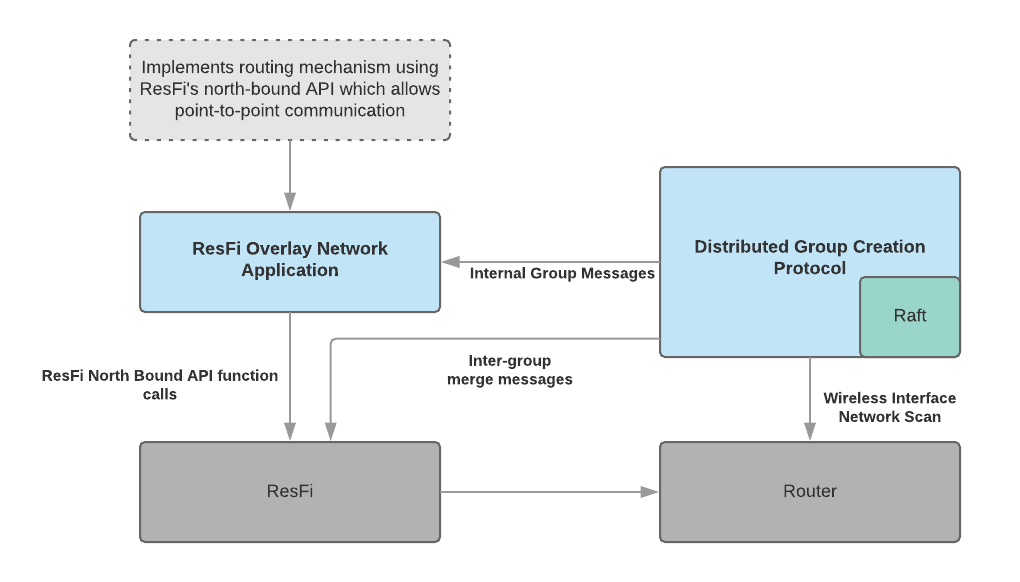
\includegraphics[width=\textwidth]{Images/dgcpoverview.png}
		\caption{Architectural overview of protocol components }%
		\label{fig:dgcpoverview}%
\end{figure}




\section{Protocol implementation}
